\subsection{Simple logic synthesis using Z3 and Apollo Guidance Computer}

\renewcommand{\CURPATH}{synth/logic/simple_and_Apollo}

What a smallest possible logic circuit is possible for a given truth table?

Let's try to define truth tables for inputs and outputs and find smallest circuit.
This program is almost the same as I mentioned earlier: \ref{synth_mult}, but reworked slightly:

\lstinputlisting[style=custompy]{\CURPATH/logic.py}

I could generate only small circuits maybe up to $\approx 10$ gates, but this is interesting nonetheless.

Also, I've always wondering how you can do something usable for Apollo Guidance Computer,
which had only one single gate: NOR3?
See also its schematics: \url{http://klabs.org/history/ech/agc_schematics/}.
The answer is De Morgan's laws, but this is not obvious.

INPUTS[] has all possible bit combinations for all inputs, or all possible truth tables. OUTPUTS[] has truth table for each output.
All the rest is processed in bitsliced manner.
Given that, the resulting program will work on 4/8/16-bit CPU and will generate defined OUTPUTS for defined INPUTS.
Or, this program can be treated just like a logic circuit.

\subsubsection{AND gate}

How to build 2-input AND gate using only OR's and NOT's?

\begin{lstlisting}
INPUTS=[0b1100, 0b1010]
OUTPUTS=[0b1000]
BITS=4
avail=[I_OR, I_NOT]

...

r0=input                 1100
r1=input                 1010
r2=NOT r1                0101
r3=NOT r0                0011
r4=OR r3, r2             0111
r5=NOT r4                1000
\end{lstlisting}

This is indeed like stated in De Morgan's laws: $x \wedge y$ is equivalent to $\neg (\neg x \vee \neg y)$.
Can be used for obfuscation?

Now using only NOR3 gate?

\begin{lstlisting}
avail=[I_NOR3]

...

r0=input                 1100
r1=input                 1010
r2=NOR3 r1, r1, r1       0101
r3=NOR3 r2, r0, r0       0010
r4=NOR3 r3, r2, r2       1000
\end{lstlisting}

\subsubsection{XOR gate}

How to build 2-input XOR using only OR's and NOT's?

\begin{lstlisting}
INPUTS=[0b1100, 0b1010]
OUTPUTS=[0b0110]
BITS=4
avail=[I_OR, I_NOT]

...

7 instructions
r0=input                 1100
r1=input                 1010
r2=OR r1, r0             1110
r3=NOT r2                0001
r4=OR r0, r3             1101
r5=NOT r4                0010
r6=OR r1, r3             1011
r7=NOT r6                0100
r8=OR r5, r7             0110
\end{lstlisting}

... using only AND's and NOT's?

\begin{lstlisting}
avail=[I_AND, I_NOT]
...
r0=input                 1100
r1=input                 1010
r2=NOT r1                0101
r3=AND r1, r0            1000
r4=NOT r3                0111
r5=NOT r0                0011
r6=AND r2, r5            0001
r7=NOT r6                1110
r8=AND r4, r7            0110
\end{lstlisting}

... using only NOR3 gates?

\begin{lstlisting}
avail=[I_NOR3]
...
r0=input                 1100
r1=input                 1010
r2=NOR3 r1, r1, r1       0101
r3=NOR3 r0, r0, r1       0001
r4=NOR3 r0, r2, r3       0010
r5=NOR3 r2, r4, r2       1000
r6=NOR3 r3, r5, r3       0110
\end{lstlisting}

\subsubsection{Full-adder}

According to Wikipedia, \href{https://en.wikipedia.org/wiki/Adder_(electronics)}{full-adder}
can be constructed using two XOR gates, two AND gates and one OR gate.
But I had no idea 3 XORs and 2 ANDs can be used instead:

\begin{lstlisting}
INPUTS=[0b11110000, 0b11001100, 0b10101010]
OUTPUTS=[0b11101000, 0b10010110] # carry-out, sum
BITS=8
avail=[I_AND, I_OR, I_XOR, I_NOT]

...

5 instructions
r0=input                 11110000
r1=input                 11001100
r2=input                 10101010
r3=XOR r2, r1            01100110
r4=AND r0, r3            01100000
r5=AND r2, r1            10001000
r6=XOR r4, r5            11101000
r7=XOR r0, r3            10010110
\end{lstlisting}

... using only NOR3 gates:

\begin{lstlisting}
avail=[I_NOR3]
...
8 instructions
r0=input                 11110000
r1=input                 11001100
r2=input                 10101010
r3=NOR3 r0, r0, r1       00000011
r4=NOR3 r2, r3, r1       00010000
r5=NOR3 r3, r2, r0       00000100
r6=NOR3 r3, r0, r5       00001000
r7=NOR3 r5, r2, r4       01000001
r8=NOR3 r3, r4, r1       00100000
r9=NOR3 r3, r5, r4       11101000
r10=NOR3 r8, r7, r6      10010110
\end{lstlisting}

\subsubsection{POPCNT}

Smallest circuit to count bits in 3-bit input, producing 2-bit output:

\begin{lstlisting}
INPUTS=[0b11110000, 0b11001100, 0b10101010]
OUTPUTS=[0b11101000, 0b10010110] # high, low
BITS=8
avail=[I_AND, I_OR, I_XOR, I_NOT]
...
5 instructions
r0=input                 11110000
r1=input                 11001100
r2=input                 10101010
r3=XOR r2, r1            01100110
r4=AND r0, r3            01100000
r5=AND r2, r1            10001000
r6=XOR r4, r5            11101000
r7=XOR r0, r3            10010110
\end{lstlisting}

... using only NOR3 gates:

\begin{lstlisting}
avail=[I_NOR3]
...
8 instructions
r0=input                 11110000
r1=input                 11001100
r2=input                 10101010
r3=NOR3 r0, r0, r1       00000011
r4=NOR3 r2, r3, r1       00010000
r5=NOR3 r3, r2, r0       00000100
r6=NOR3 r3, r0, r5       00001000
r7=NOR3 r5, r2, r4       01000001
r8=NOR3 r3, r4, r1       00100000
r9=NOR3 r3, r5, r4       11101000
r10=NOR3 r8, r7, r6      10010110
\end{lstlisting}

\subsubsection{Circuit for a central "g" segment of 7-segment display}

\begin{figure}[H]
\centering
\frame{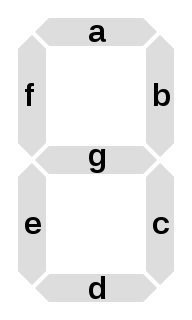
\includegraphics[scale=0.6]{\CURPATH/192px-7-segment_labeled.png}}
\end{figure}

(The image taken from \href{https://commons.wikimedia.org/wiki/File:7-segment_labeled.svg}{Wikipedia}.)

I couldn't find a circuit for the all 7 segments, but found for one, a central one ("g").
Yes, encoders like these are usually implemented using a ROM.
But I always been wondering, how to do this using only gates.

The truth table for "g" segment I've used from this table:

\begin{figure}[H]
\centering
\frame{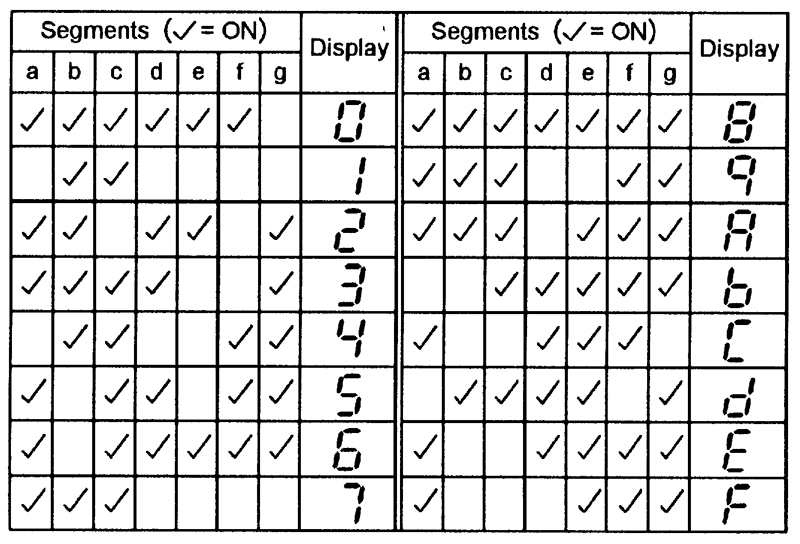
\includegraphics[scale=0.6]{\CURPATH/NV_0501_Marston_Figure02.jpg}}
\end{figure}

(The image taken from \url{http://www.nutsvolts.com}.)

\begin{lstlisting}
INPUTS=[0b1111111100000000, 0b1111000011110000, 0b1100110011001100, 0b1010101010101010]
# "g" segment, like here: http://www.nutsvolts.com/uploads/wygwam/NV_0501_Marston_Figure02.jpg
OUTPUTS=[0b1110111101111100] # g
BITS=16
avail=[I_AND, I_OR, I_XOR, I_NOT]
...
5 instructions
r0=input                 1111111100000000
r1=input                 1111000011110000
r2=input                 1100110011001100
r3=input                 1010101010101010
r4=AND r3, r1            1010000010100000
r5=XOR r4, r0            0101111110100000
r6=XOR r4, r2            0110110001101100
r7=XOR r5, r1            1010111101010000
r8=OR r7, r6             1110111101111100
\end{lstlisting}

Using only NOR3 gates:

\begin{lstlisting}
avail=[I_NOR3]
...
8 instructions
r0=input                 1111111100000000
r1=input                 1111000011110000
r2=input                 1100110011001100
r3=input                 1010101010101010
r4=NOR3 r1, r1, r1       0000111100001111
r5=NOR3 r3, r3, r4       0101000001010000
r6=NOR3 r2, r0, r0       0000000000110011
r7=NOR3 r6, r6, r5       1010111110001100
r8=NOR3 r4, r0, r7       0000000001110000
r9=NOR3 r8, r7, r2       0001000000000011
r10=NOR3 r0, r8, r4      0000000010000000
r11=NOR3 r9, r10, r10    1110111101111100
\end{lstlisting}

